\ylDisplay{Diaprojektor} % Ülesande nimi
{EFO žürii} % Autor
{piirkonnavoor} % Voor
{2017} % Aasta
{P 6} % Ülesande nr.
{3} % Raskustase
{
% Teema: Valgusõpetus
\ifStatement
Diaprojektori objektiivi fookuskaugus on $40$ $mm$. Diapositiivi näitamisel on ekraanile tekkiv kujutis diapositiivist $80$ korda suurem. Kui kaugele objektiivi fokaaltasandist on paigutatud diapositiiv? Diapositiiv on sarnane fotoga, on üks kaader filmilindist, millel esemete värvused vastavad nende tegelikele värvustele ja mida diaprojektori abil saab projitseerida ekraanile.
\fi
\ifHint
Ülesande lahendamiseks tuleb koostada joonis ning lahendada see sarnaste kolmnurkade seostega.
\fi
\ifSolution
\begin{center}
	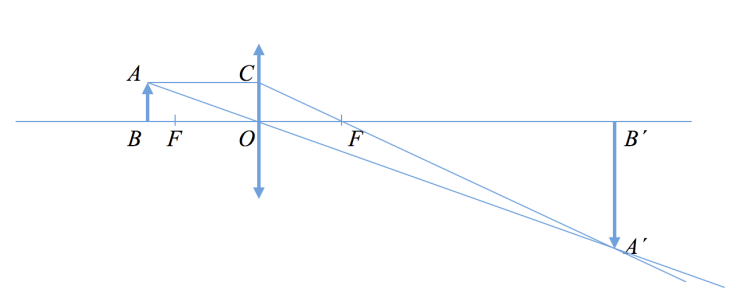
\includegraphics[width=0.5\linewidth]{2017-v2p-06-lah.PNG}
\end{center}
Tähistame slaidi kauguse objektiivist $BO$ tähega $a$, kujutise kauguse objektiivist $OB'$ tähega $k$, objektiivi fookuskauguse tähega $f$, slaidi $AB$ kõrguse tähega $h$ ja kujutise $A'B'$ kõrguse tähega $H$.\\
Kolmnurgad $ABO$ ja $OB'A$’ on sarnased, nurkade võrdsuse tunnuse järgi. \\
Kolmnurkade sarnasusest tuleneb, et $\frac{H}{h} = \frac{k}{a}$. \\
Kuna kujutise suurendus $\frac{H}{h}$ on $80$ korda, siis $k = 80$ $a$. \\
Eseme kõrgus $AB$ on võrdne lõiguga $OC$. \\
Sarnastest kolmnurkadest $OCF$ ja $OB'A'$  saame, et
\begin{center}
$\frac{H}{h} = \frac{k - f}{f}$ ehk $k = 81f$. 
\end{center}
Asendame saadud $k$ väärtuse seosesse $k = 80a$, saame 
\begin{center}
$a = \frac{k}{80} = \frac{81}{80}f$. 
\end{center}
Asendades fookuskauguse väärtuse, saame, et $a = 40,5$ mm. Kuna fookuskaugus on $40$ mm, asub slaid fokaaltasandist $0,5$ mm kaugusel.
\fi
}